\documentclass{standalone}
\usepackage{tikz}
\begin{document}
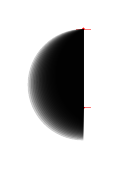
\begin{tikzpicture}
\usetikzlibrary{calc}

% draws lens of height 1 with bends of given lengths
% bend-left, bend-right
\newcommand\lens[2]{
    \pgfmathsetmacro\aaa{90-2*atan2(#1,.5)};
    \fill (0,+.5) arc ((\aaa)+90:270-(\aaa):{sqrt(0.25+(#1)^2)/cos((\aaa))});
    % \pgfmathsetmacro\bbb{90-2*atan2(#2,.5)};
    % \fill (0,-.5) arc (\bbb-90:90-\bbb:{sqrt(0.25+#2^2)/cos(\bbb)});
}

\draw[|-|,red,draw opacity=.5] (0,-.5) -- (0,.5);
\draw[red] (0,+.5) circle (.01);
\draw[red] (0,-.5) circle (.01);
\begin{scope}[fill opacity=.2]
    % \lens{1/10}{.5}
    % \lens{2/10}{.4}
    % \lens{3/10}{.3}
    % \lens{4/10}{.2}
    % \lens{5/10}{.1}
    \foreach \i in {1,...,50}{
        \lens{\i/100}{.5}
    }
\end{scope}

% position, radius, bend, back-color, fron-color
% \newcommand\custommoon[5]{
    % \fill[#4] (#1) circle (#2);
    % \fill[#5] ($(#1)+(0,#2)$) arc (90:-90:#2) to[bend right=#3] ($(#1)+(0,#2)$);
    % \draw (#1) circle (#2);
% }

% \draw[densely dotted] (0,0) circle (3) (0,0) circle (2);
% \foreach \ang in {0,45,...,359}{
    % \draw[dotted] (0,0) to (\ang:3);
% }
% \custommoon{0:0}{1}{0}{white}{gray}

% \foreach \ang in {0,45,...,359}{
    % \custommoon{\ang:2}{.3}{0}{white}{gray}
% }
% \draw[fill=white] (0:3) circle (.3);
% \draw[fill=gray] (180:3) circle (.3);
% \foreach \ang in {45,90,135}{
    % \custommoon{\ang:3    }{.3}{90-\ang}{white}{gray}
    % \custommoon{\ang+180:3}{.3}{90-\ang}{gray}{white}
% }

\end{tikzpicture}
\end{document}
